%------------------------------------------------
%
% Tools.tex 
%
% This section illustrates the tools used by
% the service desk staff
%------------------------------------------------
\section[Strumenti di lavoro]{strumenti di lavoro}
\label{sd-tools}
Il proponente intende proporre, come \english{software} di lavoro per i membri del \english{Service Desk}, l'adozione di \keyword{\href{http://www.samanage.com/}{samanage}}.

Samanage è una piattaforma per \english{Service Desk} e la gestione degli \english{assets} appoggiata nel \english{cloud} che riduce il carico di lavoro al \english{Service Desk Manager} e aiuta a fornire un servizio \keyword{veloce} e di \keyword{qualità}.

Essendo una piattaforma appoggiata nel \english{cloud} essa possiede le proprietà precedentemente discusse ed offre agli utilizzatori le seguenti funzionalità:

\begin{itemize}
\item{servizio di \english{Service Desk};}
\item{gestione di contratti e licenze;}
\item{gestione della \ac{Knowledge-Base};}
\item{analisi dei report;}
\item{gestione utenti di \ac{Active-Directory};}
\item{gestione degli \english{assets};}
\item{gestione di un portale \english{self-service};}
\item{rilevazione di possibili anomalie (rischi);}
\item{gestione di problemi e cambiamenti;}
\item{gestione del \english{Service Catalogue};}
\item{gestione dei documenti di \ac{Service-Level-Management};}
\end{itemize}

\subsection[Servizio di IT Service Desk]{servizio di IT service desk}
\label{sd-samanage-sd-service}
Samanage offre le funzionalità di un moderno \english{Service Desk} che consente di avere maggiore e miglior comunicazione con gli utenti, ottimizzare le richieste di supporto al fine di fornire un miglior servizio.

La piattaforma è basata sulle \english{best-practice} \ac{Information-Technology-Infrastructure-Library} per aiutare ad organizzare, gestire le priorità e risolvere efficientemente gli incidenti. Include strumenti a supporto al processo di \ac{Change-Management}, gestione della \ac{Knowledge-Base} e del \english{Service Catalog}.

Samanage offre inoltre la possibilità sottoporre gli utenti a brevi questionari che restituiscono un \english{feedback} al \english{Service Desk Manager}. L'analisi di questi \english{feedback} consente alla funzionalità di scalare qualora il servizio offerto non fosse in linea con quanto progettato o con le aspettative degli utenti.

\subsection[Gestione di contratti e e licenze]{gestione di contratti e licenze}
\label{sd-samanage-contract-license}
Samanage permette di gestire in un unico punto tutte le licenze di prodotti ed i contratti \acs{Information-Technology} presenti nell'istituto.

Una apposita sezione (vedi figura \ref{sd-samanage-contract-license-img}) del \english{software} consente di avere una visione d'insieme sui differenti tipi di contratti (come \acs{Internet-Service-Provider}, \english{hosting}, ecc..) e i loro rispettivi casi d'uso. Inclusi nella banca dati vi saranno licenze \english{software}, contratti di locazione \english{hardware}, abbonamenti e contratti di manutenzione con le rispettive date di acquisto e scadenza.

\begin{figure}[htbp]
\centering
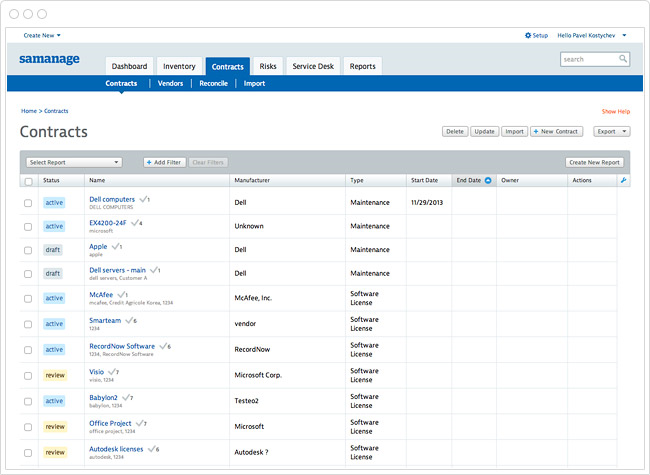
\includegraphics[scale=0.6]{Images/samanage/Contract_license.png}
\caption{Gestione di contratti e licenze}
\label{sd-samanage-contract-license-img}
\end{figure}

Permette inoltre di tenere traccia dei pagamenti effettuati a seguito di rinnovi, e di impostare dei promemoria vicino alle date di scadenza delle licenze/contratti affinché sia possibile rinnovarli senza alcuna perdita di servizio.

\subsection[Gestione della Knowledge Base e del portale self-service]{gestione della knowledge base del portale self-service}
\label{sd-samanage-knowledge-base}
Il \english{software} consente di conservare in un unico posto logico (vedi figura \ref{sd-samanage-knowledge-base-img-1}) tutte le \english{best practices} e le soluzioni a richieste comuni.

\begin{figure}[htbp]
\centering
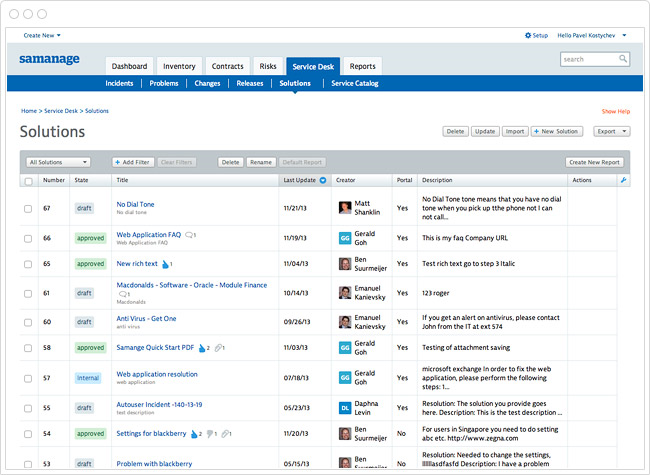
\includegraphics[scale=0.6]{Images/samanage/Knowledge_base.png}
\caption{Gestione della \ac{Knowledge-Base} per lo staff tecnico}
\label{sd-samanage-knowledge-base-img-1}
\end{figure}

Utilizzare il sistema integrato di gestione della \ac{Knowledge-Base} consente di ridurre i tempi di risoluzione dei problemi, e servire da piattaforma di condivisione della conoscenza, perché accessibile a tutti gli utenti dei servizi (vedi figura \ref{sd-samanage-knowledge-base-img-2}). 

Questo portale è il portale ``\english{self-service}'' in cui gli utenti posso accedere alle soluzioni a problemi comuni.

\begin{figure}[htbp]
\centering
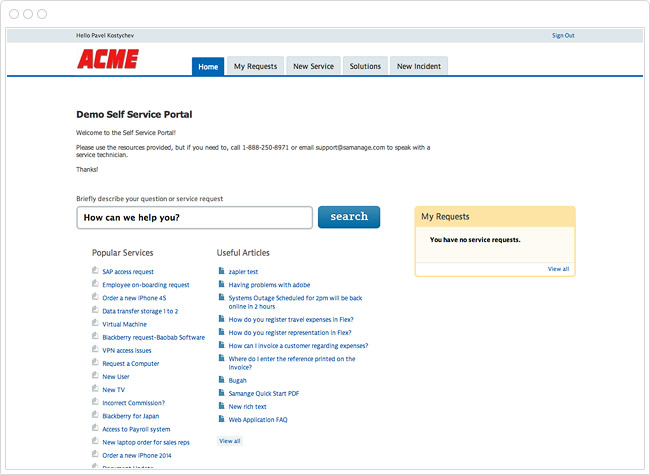
\includegraphics[scale=0.6]{Images/samanage/Knowledge_base_self_service.png}
\caption{Accesso alla \ac{Knowledge-Base} per gli utenti}
\label{sd-samanage-knowledge-base-img-2}
\end{figure}

Questo aumenta l'efficienza di supporto e aumenta la consapevolezza effettiva della conoscenza \acs{Information-Technology} in tutto l'istituto.

\subsection[Gestione ed analisi dei report]{gestione ed analisi dei report}
\label{sd-samanage-report-management}
Il \english{software} fornisce un robusto e flessibile sistema di gestione dei report e dei \english{feedback} degli utenti, che consente di mantenere sempre sotto controllo le attività svolte dallo staff tecnico.

\begin{figure}[htbp]
\centering
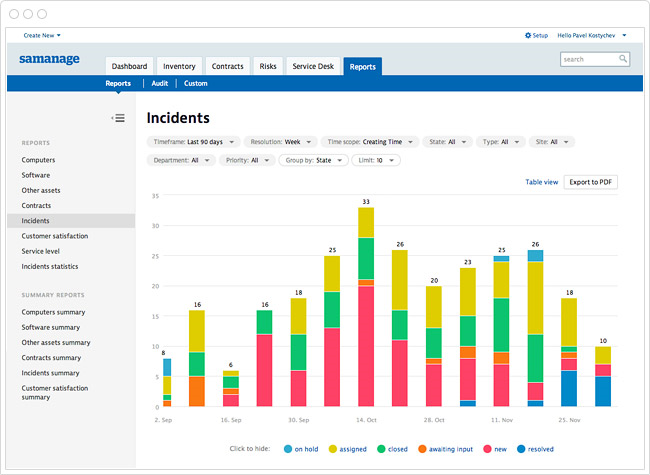
\includegraphics[scale=0.6]{Images/samanage/Report_management.png}
\caption{Gestione ed analisi di report}
\label{sd-samanage-report-management-img}
\end{figure}

E' possibile filtrare ed analizzare i dati, scoprire importanti \english{patterns} e \english{trends} che possono impattare le \english{performance} dell'ambiente \acs{Information-Technology} (vedi figura \ref{sd-samanage-report-management-img}).

\subsection[Integrazione con Active Directory]{integrazione con Active Directory}
\label{sd-samanage-active-directory}
\acf{Active-Directory} è uno dei più popolari metodi per gestire i \english{files} degli utenti, i permessi e le informazioni di contatto all'interno di un dominio \english{Microsoft Windows}.

Samanage rende semplice la sincronizzazione dell'\ac{Active-Directory} dell'istituto consentendo di controllarlo da un unico posto centralizzato.

\subsection[Gestione degli assets]{gestione degli assets}
\label{sd-samanage-assets-management}
Con il modulo di \acs{Information-Technology} \ac{Asset-Management} lo staff tecnico è in grado di controllare più agevolmente lo scenario tecnologico presente nell'istituto.

Questo modulo offre potenti strumenti e funzionalità che comprendono un sistema continuo per tenere traccia dell'inventario \english{hardware} e \english{software} dell'istituto, compresi i \acs{Personal-Computer}, server, \english{laptop}, dispositivi \english{mobile}, dispositivi di rete e qualsiasi altro \english{asset} tecnologico presente. In figura \ref{sd-samanage-asset-management-img} è possibile vedere la schermata che permette la gestione degli \english{asset}.

\begin{figure}[htbp]
\centering
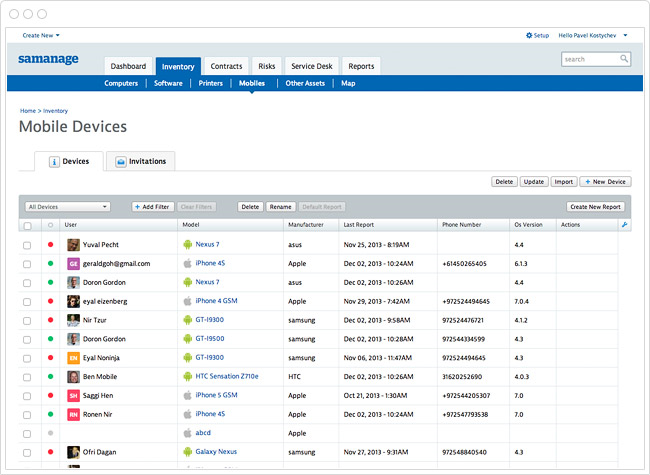
\includegraphics[scale=0.6]{Images/samanage/Asset_management.png}
\caption{Gestione degli \english{asset}}
\label{sd-samanage-asset-management-img}
\end{figure}

Il modulo aiuta inoltre a garantire la conformità del \english{software}, aumentare la sicurezza e ridurre al minimo i costi attraverso una soluzione di semplice utilizzo per la gestione degli \english{asset}.

\subsection[Gestione di possibili anomalie]{gestione di possibili anomalie}
\label{sd-risk-management}
La gestione del rischio \acs{Information-Technology} può e deve essere considerato come un componente primario di un più ampio scenario di gestione del rischio aziendale, e quindi è desiderabile investire in un sistema di controllo efficace.

La soluzione \english{software} proposta consente di gestire le situazioni di rischio aiutando lo staff tecnico a concentrarsi sulle aree che richiedo maggior attenzione nell'ambiente \acs{Information-Technology}.

\begin{figure}[htbp]
\centering
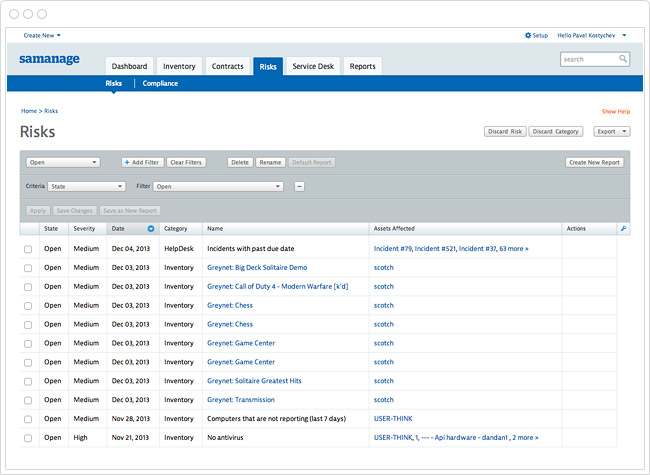
\includegraphics[scale=0.6]{Images/samanage/Risk_management.png}
\caption{Schermata che consente di tenere le problematiche sotto controllo}
\label{sd-samanage-risk-management-img}
\end{figure}

Esso include un motore di rilevamento del rischio che analizza costantemente i dati memorizzati nella sua banca dati (come per esempio l'inventario delle attività o richieste al \english{Service Desk}) e cerca modelli problematici. Se ne dovesse rilevare alcuni saranno in automatico aperte delle notifiche (vedi figura \ref{sd-samanage-risk-management-img}) che possono essere viste dal personale del \english{Service Desk}.

\subsection[Gestione di problemi e cambiamenti]{gestione di problemi e cambiamenti}
\label{sd-problem-change-management}
La soluzione \english{software} proposta fornisce strumenti per la gestione e l'approvazione delle modifiche ai \ac{Configuration-Item} presenti nell'ambiente \acs{Information-Technology}.

Questo consente di trovare soluzioni permanenti ai problemi e prevenire gli incidenti ripetuti che causano interruzioni del servizio.

Attraverso gli strumenti di approvazione delle modifiche possiamo garantire che le modifiche effettuate dal processo di \ac{Change-Management} siano in linea con la strategia aziendale complessiva prima della loro messa in produzione.

\subsection[Gestione del service catalogue]{gestione del service catalogue}
\label{sd-service-catalogue-management}
Samanage permette la gestione di un \english{Service Catalogue} in linea con le \english{best practice} \ac{Information-Technology-Infrastructure-Library}.

\begin{figure}[htbp]
\centering
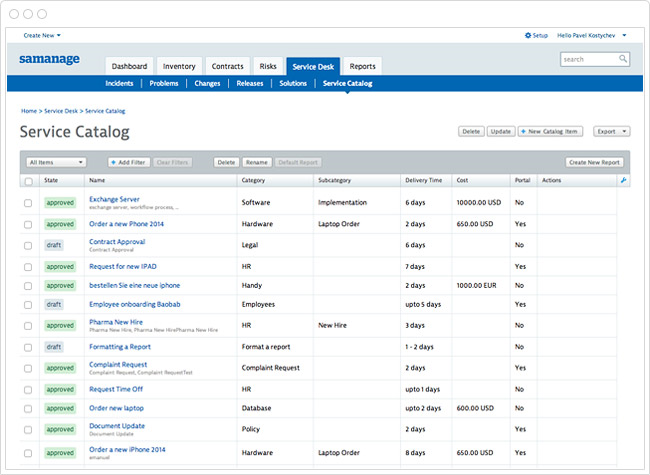
\includegraphics[scale=0.6]{Images/samanage/Service_catalogue.png}
\caption{Schermata che visualizza i servizi offerti dal dipartimento}
\label{sd-samanage-service-catalogue-img}
\end{figure}

Sarà possibile definire e pubblicare, all'interno del portale (vedi figura \ref{sd-samanage-service-catalogue-img}), i servizi disponibili con le relativi soluzioni per gestire al meglio i carichi di lavoro.

Questo incoraggia gli utenti all'uso del portale \english{self-service} consentendo quindi loro di effettuare delle richieste di servizio da un elenco prestabilito, agevolando cosi il lavoro dello staff di \english{Service Desk}.

\subsection[Gestione dei documenti di SLM]{gestione dei documenti di SLM}
\label{sd-sla-management}
Gli accordi sui livelli di servizio offerti sono una parte importante della gestione del dipartimento \acs{Information-Technology}.

Gli \ac{Service-Level-Agreement} definiscono come viene effettuata la misura delle \english{performance}, la gestione dei problemi, le garanzie, i tempi di risposta ecc. Con adeguati obiettivi di \ac{Service-Level-Agreement} il dipartimento sarà in grado di garantire ottimi livelli di servizio ed assicurare che il servizio offerto rispetti gli accordi.

\begin{figure}[htbp]
\centering
\includegraphics[scale=0.6]{Images/samanage/Service_level_management.png}
\caption{Schermata che consente di tracciare gli \ac{Service-Level-Management}}
\label{sd-samanage-service-level-management-img}
\end{figure}

La soluzione proposta consente di gestire in unico posto (vedi figura \ref{sd-samanage-service-level-management-img}) tutti i documenti e tracciarne le eventuali modifiche affinché nulla vada perso o sia lasciato al caso.




























